Debido a la dificultad computacional del problema, no existe a\'un una soluci\'on exacta de tiempo polinomial, y a pesar de que nos entretuvimos
discutiendo, nosotros no pudimos encontrarla tampoco. En su defecto implementamos un algoritmo de backtracking que recorre todos los caminos
posibles de $u$ a $v$ y se queda con el de menor $\omega_2$ tal que $\omega_1 \leq K$. 

El algoritmo funciona de la siguiente manera: en un momento dado va a tener construido un camino $P = [v_1 = u, \dots, v_{i-1}]$, y toma un nodo
$v_i$ aun no visitado de la adyacencia de $v_{i-1}$, lo marca como visitado y lo agrega a $P$. Si $\omega_1(P)$ se pasa de $K$, este camino ya no
nos sirve y no sigo avanzando en la recursión. Caso contrario, se llama a la recursión sobre el camino aumentado.

En el caso en que $v_i$ = $v$, sabemos que tenemos una solución candidata. Comparamos $\omega_2(P)$ con el menor $\omega_2$ entre las soluciones
candidatas, y si es mejor solución, se guarda. Cuando hemos llegado a $v$ no hace falta llamar a la recursión.

Siempre antes de retornar tras explorar un nodo de un camino, se lo marca como no visitado, para que pueda ser recorrido en otros caminos que se
recorran.

A continuaci\'on, escribimos el pseudoc\'odigo de la funci\'on \texttt{main}.
\begin{algorithm}[H]
\caption{$main$()}
\begin{algorithmic}[1]
  \State Camino mejorSolucion
  \State $\omega_2$(mejorSolucion) $\leftarrow$ $\infty$
  \State Camino ramaActual $\leftarrow$ []
  \For{i \textbf{en} 1 \textbf{a} n}
    \State visitados[i] = False
  \EndFor
  \State backtrack( u, null )
  \If{$\omega_2$(mejorSolucion) $<$ $\infty$}
    \State imprimir(mejorSolucion)
  \Else{}
    \State imprimir("no")
  \EndIf
\end{algorithmic}
\end{algorithm}

\begin{algorithm}[H]
\caption{$backtrack$(Nodo actual, Nodo padre)}
\begin{algorithmic}[1]
  \State ramaActual.push( actual )
  \State visitados[actual] $\leftarrow$ true
  \If{$\omega_1$(ramaActual) $< K$}
    \If{actual = v \textbf{and} $\omega_2$(ramaActual) $< \omega_2$(mejorSolucion)} 
      \State mejorSolucion $\leftarrow$ ramaActual
      \ElsIf{actual $\neq$ v \textbf{and} $\omega_1$(ramaActual) $\leq$ K}
      \For{\textbf{cada} Nodo n \textbf{en} adyacentes( actual ) }
	\If{\textbf{no} visitado[n] }
	  \State backtrack( n, actual )
	\EndIf
      \EndFor
    \EndIf
  \EndIf
  \State ramaActual.pop( actual )
  \State visitados[actual] $\leftarrow$ false
\end{algorithmic}
\end{algorithm}

Complejidad:

Analicemos cuantas llamadas se hacen a $backtrack$. Se exploran caminos de a los sumo $n$ nodos. El primer nodo está fijo en $u$. El segundo nodo
pertenece a la adyacencia del primero, que en peor caso tiene tamaño $n - 1$. El tercero pertenece a la adyacencia del segundo, que no hayan sido
visitados, cuyo tamaño es a lo sumo $n - 2$. Y asi sucesivamente. En peor caso se llama a $backtrack$ $n!$ veces.

Analicemos el cómputo que se realiza en cada llamada a $backtrack$. Preguntar si un nodo está visitado es acceder a un arreglo en forma constante.
El costo de una función de peso asociada a un camino se va acumulando a medida que se agregan nodos. El costo se guarda y se puede acceder en
forma constante. Lo queda por estudiar es la complejidad del ciclo $for$ que recorre la adyacencia del nodo visitado. Guardamos una lista de
adyacencia por lo que podemos recorrer la adyacencia de cualquier nodo con complejidad lineal en relación a su tamaño. El tamaño de la adyacencia
es a lo sumo $m$. Para cada nodo adyacente se efectúan operaciones constantes, a excepción de las llamadas a $backtrack$. El costo de estas
llamadas lo estamos calculando por separado.

En definitiva hacemos $O(n!)$ llamadas a una función que de por si toma $O(m)$ operaciones. La complejidad del algoritmo es $O(m*n!)$.

Experimentación:

Generamos en primera instancia grafos con una cantidad de nodos pequeña - entre 3 y 15. La cantidad de aristas, es decir, la densidad del grafo,
se eligió aleatoriamente entre 0 y (n * (n - 1)) / 2, la cantidad máxima posible. La distribución de las aristas, sus pesos, y el valor de $k$
también se eligieron de forma aleatoria.

A continuación presentamos los tiempos de ejecución de nuestro algoritmo frente a estas instancias. 

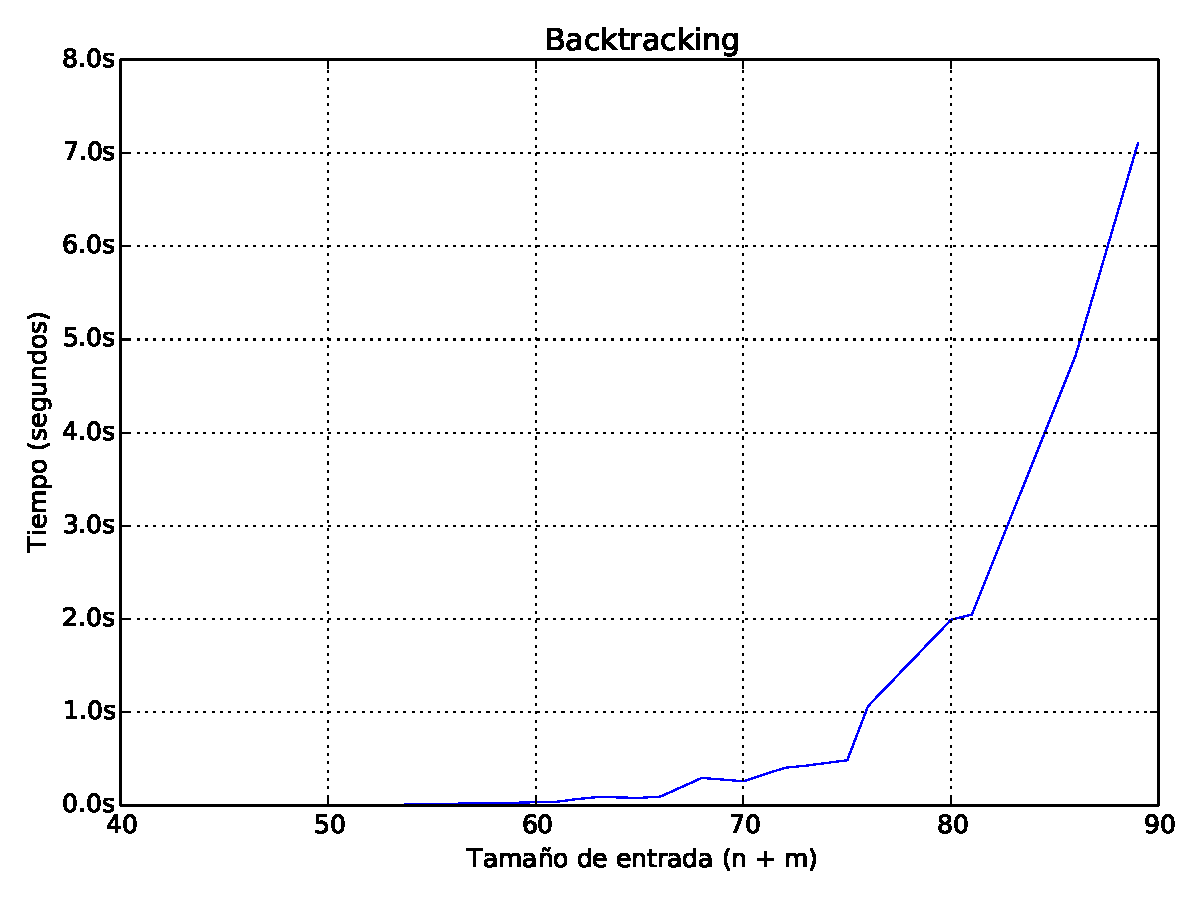
\includepdf[pages={1}]{imagenes/backtracking-aleatorio.pdf}

Para tamaños de grafo menores que 40, los tiempos de ejecución fueron despreciables. Se puede apreciar el carácter exponencial del tiempo de
ejecución de nuestro algoritmo en función del tamaño de entrada.

\fixme{Hacer mas experimentación? dejando fijo n y m? fue dificil sacar resultados para eso}
